%versi 2 (8-10-2016)
\chapter{Landasan Teori}
\label{chap:teori}
Pada bab ini dijelaskan dasar-dasar teori mengenai \textit{Wireless Sensor Network}, Reliable Data Transfer di WSN, dan pemrograman pada WSN.

\section{Wireless Sensor Network}
\label{sec:wsn}
\textit{Wireless Sensor Network} (WSN) merupakan jaringan nirkabel yang terdiri dari sekumpulan node sensor yang diletakan pada suatu tempat dan memiliki kemampuan untuk mengukur kondisi lingkungan sekitar(\textit{sensing}), melakukan komputasi dan dilengkapi dengan alat komunikasi \textit{wireless} untuk komunikasi antara node sensor. Sensor ini akan mengumpulkan data dari kondisi lingkungannya, seperti: cahaya, suara, kelembapan, getaran, gerakan, temperatur, tekanan udara, kualitas air, komposisi tanah, dan lain-lain. Data ini kemudian dapat dikirimkan langsung ke \textit{base station} atau melalui node sensor tetangganya hingga sampai ke \textit{base station} sebagai pusat untuk dikelola.

\subsection{Penerapan Wireless Sensor Network}
Pada awalnya \textit{sensor network} (jaringan sensor) digunakan dalam teknologi militer untuk mendeteksi musuh di laut dan di darat. Semakin lama node sensor ini banyak dikembangkan untuk membantu berbagai bidang kehidupan manusia. Pemanfaatan WSN pada kehidupan manusia dapat dilihat pada ilustrasi Gambar~\ref{fig:smartworld}. Berikut adalah beberapa penerapan WSN:
\begin{itemize}
\item Bidang Militer\\
Pada bidang militer WSN digunakan untuk melakukan pemantauan musuh dan melindungi wilayah. WSN juga dapat digunakan untuk mendeteksi serangan dari musuh.

\item Monitoring area\\
Pada \textit{monitoring area}, node sensor akan disebar pada suatu tempat yang akan di monitoring. Saat node sensor mendeteksi kejadian(panas, tekanan, dan lain-lain) pada suatu tempat, data akan dikirimkan ke \textit{base station} untuk ditentukan tindakan selanjutnya.

\item Bidang Transportasi\\
Pada bidang transportasi, WSN digunakan untuk mendeteksi arus lalu lintas secara aktual yang nantinya akan disampaikan kepada pengendara seperti kemacetan lalu lintas. 

\item Bidang Kesehatan\\
WSN dapat digunakan pada aplikasi kesehatan seperti membantu pada disabilitas, monitoring pasien, diagnosis, pengaturan penggunaan obat, dan pelacakan dokter dan pasien di rumah sakit.

\item Deteksi Lingkungan\\
Deteksi lingkungan yang dapat dilakuan antara lain deteksi gunung berapi, polusi udara, kebakaran hutan, efek rumah kaca, dan deteksi longsor.

\item Monitoring Struktur\\
WSN dapat melakukan deteksi pergerakan bangunan dan infrastruktur seperti jembatan, \textit{flyover}, terowongan dan fasilitas lain tanpa mengeluarkan biaya untuk melakukan dektesi manual dengan mendatangi tempatnya secara langsung.

\item Bidang Pertanian\\
Pada bidang pertanian dapat membantu pengelola pertanian untuk pemantauan penggunaan air dalam irigasi dan mengelola buangan pertanian mereka.
\end{itemize}

\begin{figure} [H]
	\centering  
	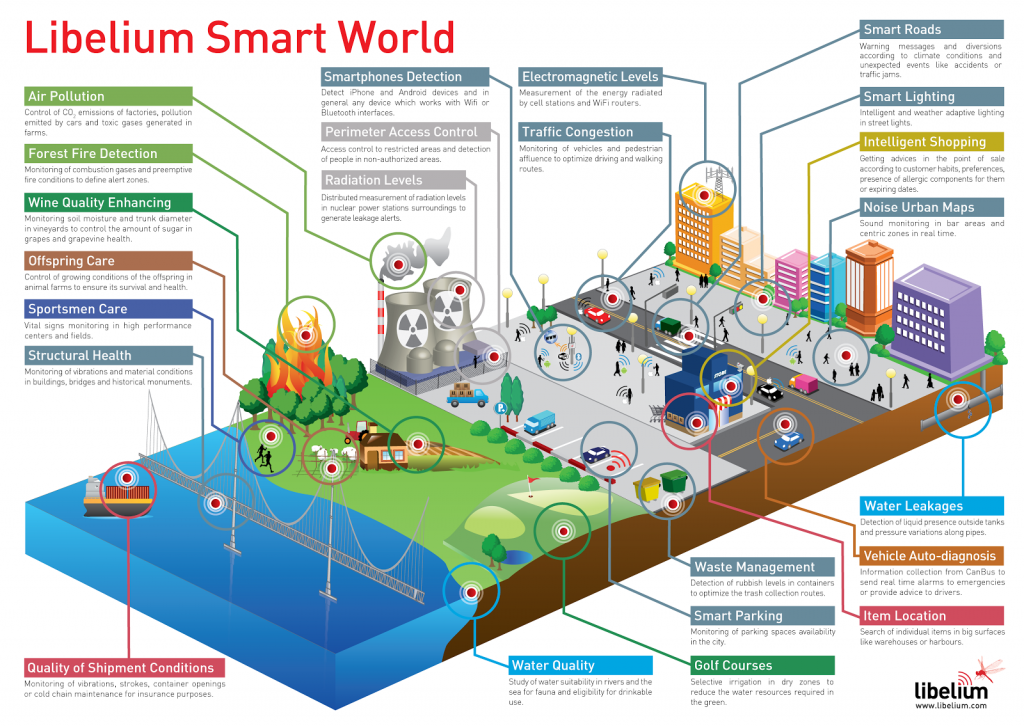
\includegraphics[scale=0.3]{libelium_smart_world}  
	\caption[Ilustrasi Pemanfaatan \textit{Wireless Sensor Network}]{Ilustrasi Pemanfaatan \textit{Wireless Sensor Network}} 
	\label{fig:smartworld} 
\end{figure} 

\subsection{Node Sensor}
\subsubsection{Struktur Node Sensor}
Setiap node sensor memiliki kemampuan deteksi, komputasi dan komunikasi. Node sensor memiliki lima komponen utama yaitu \textit{controller}, \textit{memory}, \textit{sensor and actuator}, \textit{communication device}, dan \textit{power supply}, (Gambar~\ref{fig:structure_sensor_node}). Semua komponen akan bekerja secara seimbang dalam melakukan \textit{sensing}, komputasi, komunikasi, dan menjaga penggunaan energi seminimal mungkin. 

\begin{figure} [H]
	\centering  
	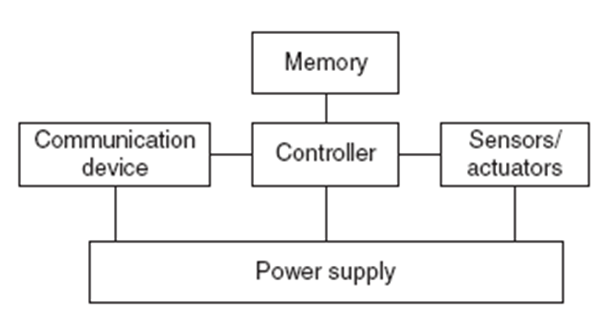
\includegraphics[scale=0.3]{structure_sensor_node}  
	\caption[Struktur Node Sensor]{Struktur Node Sensor} 
	\label{fig:structure_sensor_node} 
\end{figure} 

\subsubsection{Controller}
\textit{Controller} adalah inti utama pada node sensor. \textit{Controller} mengumpulkan data dari sensor dan memproses data tersebut hingga menentukan kapan dan kemana data tersebut dikirim. \textit{Controller} menerima data dari node sensor lain. Pada \textit{controller} biasanya terdapat \textit{microcontroller} atau \textit{microprocessor} yang mengatur dan melakukan komputasi data dari node sensor. \textit{Microcontroller} ini juga dapat mengurangi penggunaan energi dengan adanya \textit{sleep states} yang berarti hanya bagian dari controller saja yang aktif.

Beberapa \textit{microcontroller} yang digunakan dalam \textit{Wireless Sensor Node}:
\begin{itemize}
	\item Intel StrongARM (32-bit RISC, up to 206 MHz)
	\item Texas Instrument MSP 430 (16-bit RISC, up to 4 MHz,RAM 2-10 kB)
	\item Atmel Atmega 128L (8-bit)
\end{itemize}

\subsubsection{Memory}
\textit{Random Access Memory} (RAM) digunakan untuk menyimpan sementara hasil yang didapat dari sensor. RAM juga menyimpan sementara paket dari node sensor lain. Jika node sensor mati atau energi habis maka data pada RAM ini akan hilang. Data yang hilang saat node sensor mati merupakan salah satu kekurangan dari penggunaan RAM. Untuk itu dalam menyimpan kode program digunakanlah \textit{Read Only Memory} (ROM). ROM ini biasa disebut \textit{Electrically Erasable Programmable Read-Only Memory} (EEPROM) atau \textit{Flash Memory}.

\subsubsection{Communication Device}
\textit{Communication Device} digunakan untuk bertukar data antar node sensor. Pada aplikasi WSN, \textit{Radio Frequency(RF)} adalah media komunikasi yang paling relevan untuk saat ini. RF-based mendukung jangkauan yang jauh, memiliki data rate yang tinggi dan tidak perlu saling mengetahui posisi antara penerima dan pengirim.

Pada node sensor dibutuhkan \textit{transmitter} untuk mengirim data dan \textit{receiver} untuk menerima data. Kedua hal ini dapat digabung dan disebut dengan \textit{transceiver}. Tugas \textit{transceiver} adalah mengubah aliran \textit{bit} menjadi gelombang radio. Selain itu \textit{transceiver} juga dapat mengubah gelombang radio menjadi aliran \textit{bit}.

\subsubsection{Sensor dan Actuator}
Sensor dan Actuator adalah hal yang penting pada WSN. Tanpa sensor dan actuator maka node sensor tidak berguna dan tidak dapat digunakan. Tabel~\ref{tab:sensor} adalah jenis - jenis sensor yang dapat dimiliki node sensor. Sensor dikategorikan menjadi tiga:
\begin{enumerate}
	\item \textbf{Passive, omnidirectional sensors} Sensor ini dapat mengukur kualitas dari lingkungan fisik tempat node sensor tersebut tanpa mengubah lingkungannya. Beberapa sensor dikategori ini \textit{self-powered} yaitu sensor mendapatkan energi yang mereka butuhkan dari lingkungannya. \textit{Omnidirectional} berarti tidak ada arah pada sensor ini. Sensor akan memancarkan sinyalnya ke segala arah. Contoh sensor ini adalah termometer, sensor cahaya, sensor getaran, mikrofon, sensor kelembapan, sensor tekanan udara, sensor deteksi asap, dan lain-lain.
	\item \textbf{Passive, narrow-beam sensors} Sensor ini memiliki sifat yang sama dengan sensor \textit{Passive, omnidirectional sensors} yaitu tidak mengubah lingkungannya. Sensor ini dapat melakukan gerakan dan memiliki arah atau daerah pengukuran. Contoh dari sensor ini adalah kamera yang bisa mengukur sesuai dengan arah yang dituju.
	\item \textbf{Active Sensor} Sensor ini aktif dalam memeriksa lingkungannya. Contoh dari sensor ini adalah sonar, radar atau sensor seismik. Sensor ini menghasilkan gelombang untuk melakukan deteksi.
\end{enumerate}

\textit{Actuator} adalah penerima sinyal dan yang mengubahnya menjadi aksi fisik. \textit{Actuator} jumlahnya beragam seperti sensor.  Contoh aktuator adalah LED, yang mengubah listrik menjadi cahaya dan motor (motor elektrik) juga mengubah listrik menjadi gerakan.

\begin{table} [H]
	\centering 
	\caption{Jenis - jenis sensor yang dapat dimiliki node sensor}
	\label{tab:sensor}
	\begin{tabular}{|p{6cm}|p{9cm}|}
		\toprule
		Sensor & Penggunaan\\

		\midrule
		Accelerometer & Pergerakan 2D \& 3D untuk objek dan manusia  \\
		Acoustic emission sensor & Elastic Waves Generation\\
		Acoustic sensor   & Acoustic pressure vibration\\
		Capacitance sensor  & Solute Concentration\\
		ECG   & Heart Rate\\
		EEG  & Brain Electric Activity\\
		EMG   & Muscle Activity\\
		Electrical/electromagnetic sensor & Electrical Resistivity\\
		Gyroscope  & Angular Velocity \\
		Humidity Sensor   & Mendeteksi Humidity\\
		Infrasonic sensor  &  Gelombang untuk deteksi gempa dan volkanik\\
		Magnetic sensor   & Mendeteksi magnetik\\
		Oximeter   & Tekanan Oxigenation pada darah  \\
		pH sensor  & Tingkat Keasaman\\
		Photo acoustic spectroscopy   & Gas Sensing\\
		Piezoelectric cylinder    &  Gas Velocity\\
		Soil moisture sensor   &  Mengukur tanah\\
		Temperature sensor   & Temperatur \\
		Barometer sensor  &  tekanan air\\
		Passive infrared sensor  & Pergerakan infrared\\
		Seismic sensor   & Pergerakan Seismik (Gempa) \\
		Oxygen sensor  & Oksigen pada darah \\
		Blood flow sensor  & Gelombang ultrasonik pada darah \\

		\bottomrule
		
	\end{tabular} 
\end{table}

\subsubsection{Power Supply}
\textit{Power supply} atau sumber energi pada WSN bisa berasal dari dua cara yaitu \textbf{\textit{storing energy}} dan \textbf{\textit{energy scavenging}}. \textit{Storing energy} adalah dengan menggunakan baterai sebagai sumber energinya. Baterai yang digunakan dapat diisi ulang maupun tidak dapat diisi ulang. \textit{Energy scavenging} digunakan saat membuat WSN yang akan digunakan dalam waktu yang lama. Dibutuhkan energi yang bisa dikatakan tidak terbatas. Salah satu cara \textit{energy scavenging} adalah \textit{photovoltaics}. \textit{Photovoltaics} dapat disebut juga \textit{solar cell} yang memanfaatkan cahaya matahari dan mengubahnya menjadi energi sebagai pembangkit daya. Cara lain yang bisa digunakan adalah pemanfaatan angin dan air untuk mengerakan kincir atau turbin yang akan menghasilkan listrik dan digunakan sebagai sumber energi pada node sensor.

\subsection{Arsitektur dan Topologi Wireless Sensor Network}
Pada WSN biasanya akan terdapat banyak node sensor yang disebar pada suatu tempat. Terdapat satu atau lebih \textit{sink node} atau \textit{base station} dalam area sensing tersebut (Gambar~\ref{fig:arsitektur}). \textit{sink node} atau \textit{base station} adalah node sensor yang bertugas untuk mendapatkan data dari node sensor lain. Dalam membuat WSN perlu diperhatikan arsitektur dan topologi yang akan digunakan. Tidak semua topologi jaringan komputer dapat digunakan untuk \textit{Wireless Sensor Network}. 

Ada banyak topologi pada jaringan sensor (\textit{sensor network}). Pada jaringan sensor dengan menggunakan kabel, topologi yang sering digunakan adalah topologi \textit{star}, \textit{line}, atau \textit{bus}. Sedangkan pada jaringan sensor tanpa kabel (WSN), topologi yang biasa digunakan adalah \textit{star}, \textit{tree}, atau \textit{mesh}. 

\subsubsection{Topologi Point-to-Point}
Topologi \textit{Point-to-Point} adalah topologi yang menghubungkan dua titik (Gambar~\ref{fig:point2point}). Topologi \textit{Point-to-Point} dibagi menjadi dua yaitu \textit{permanent point-to-point} dan \textit{switched point-to-point}. \textit{Permanent point-to-point} adalah koneksi perangkat keras antara dua titik dan tidak dapat diubah. \textit{Switched point-to-point} adalah koneksi \textit{point-to-point} yang dapat berpindah antara node yang berbeda. 
\begin{figure} [H]
	\centering  
	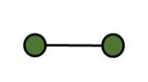
\includegraphics[scale=0.9]{point2point}  
	\caption[Topologi Point-to-Point]{Topologi Point-to-Point} 
	\label{fig:point2point} 
\end{figure} 

\subsubsection{Topologi Bus}
Topologi Bus seperti pada Gambar~\ref{fig:bus} akan terdiri dari node-node dan sebuah jalur. Setiap node akan terhubung dengan saatu jalur yang sama. Untuk mengirim data atau komunikasi akan dilakukan bergantian antar node. Kekurangan dari topologi bus ini adalah jika suatu saat jalur atau bus ini mengalami kerusakan maka setiap node tidak dapat saling berkomunikasi lagi.
\begin{figure} [H]
	\centering  
	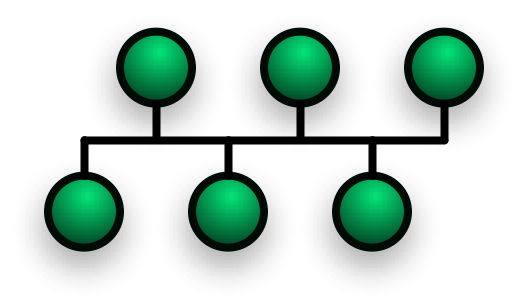
\includegraphics[scale=0.2]{bus}  
	\caption[Topologi Bus]{Topologi Bus} 
	\label{fig:bus} 
\end{figure} 

\subsubsection{Topologi Ring}
Pada Topologi \textit{Ring} node akan disusun dengan bentuk melingkar (Gambar~\ref{fig:ring}). Setiap node akan terkoneksi dengan dua node lain. Transfer data terjadi dengan cara data akan berjalan dari satu node ke node lain mengikuti jalur melingkar tersebut hingga menemukan node tujuan yang tepat. Topologi ini mudah untuk diimplementasikan tapi kekurangan dari topologi ring adalah saat ada node yang rusak maka perlu biaya lebih untuk memperbaikinya. Biasanya untuk menangani kegagalan komunikasi akibat node yang rusak, akan di atur komunikasi node tidak hanya satu arah tetapi dapat ke arah sebaliknya.
\begin{figure} [H]
	\centering  
	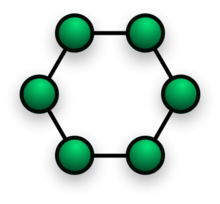
\includegraphics[scale=0.4]{ring}  
	\caption[Topologi Ring]{Topologi Ring} 
	\label{fig:ring} 
\end{figure} 

\subsubsection{Topologi Star}
Topologi \textit{Star} terdiri dari satu node yang berada di tengah biasanya berupa \textit{hub} atau \textit{switch} seperti pada Gambar~\ref{fig:star}. Setiap node akan terkoneksi dengan node yang berada di tengah ini. Saat node akan berkomunikasi dengan node lain, node tersebut harus mengirimkan data tersebut ke node yang ada ditengah dahulu dan node yang berada ditengah ini akan meneruskan data tersebut ke node tujuan. Yang paling penting pada topologi ini adalah node yang berada di tengah, karena semua komunikasi harus melalui node tersebut. Jika node tengah mengalami kerusakan maka tidak akan terjadi komunikasi antar node pada jaringan tersebut.
\begin{figure} [H]
	\centering  
	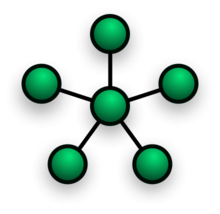
\includegraphics[scale=0.4]{star}  
	\caption[Topologi Star]{Topologi Star} 
	\label{fig:star} 
\end{figure} 

\subsubsection{Topologi Tree}
Pada Topologi \textit{Tree} node-node akan disusun secara hierarki dengan satu node yang berada pada level paling atas sebagai \textit{root node} (Gambar~\ref{fig:tree}). \textit{Root node} akan terhubung dengan satu atau lebih node level dibawahnya. Dengan Topologi \textit{Tree} lebih mudah untuk melakukan identifikasi dan meminimalisir kesalahan, namun jika \textit{tree} sudah sangat besar atau \textit{level tree} sudah sangat banyak maka akan sulit untuk melakukan konfigurasi.
\begin{figure} [H]
	\centering  
	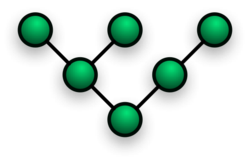
\includegraphics[scale=0.5]{tree}  
	\caption[Topologi Tree]{Topologi Tree} 
	\label{fig:tree} 
\end{figure} 

\subsubsection{Topologi Mesh}
Topologi \textit{Mesh} dibagi menjadi dua yaitu \textit{partially connected mesh} dan \textit{fully connected mesh}. Pada \textit{partially connected mesh} (Gambar~\ref{fig:mesh_partial}), node akan terhubung dengan lebih dari satu node. Pada \textit{fully connected mesh} (Gambar~\ref{fig:mesh_fully}), setiap node akan terhubung dengan semua node lain pada jaringan tersebut.
\begin{figure} [H]
	\centering  
	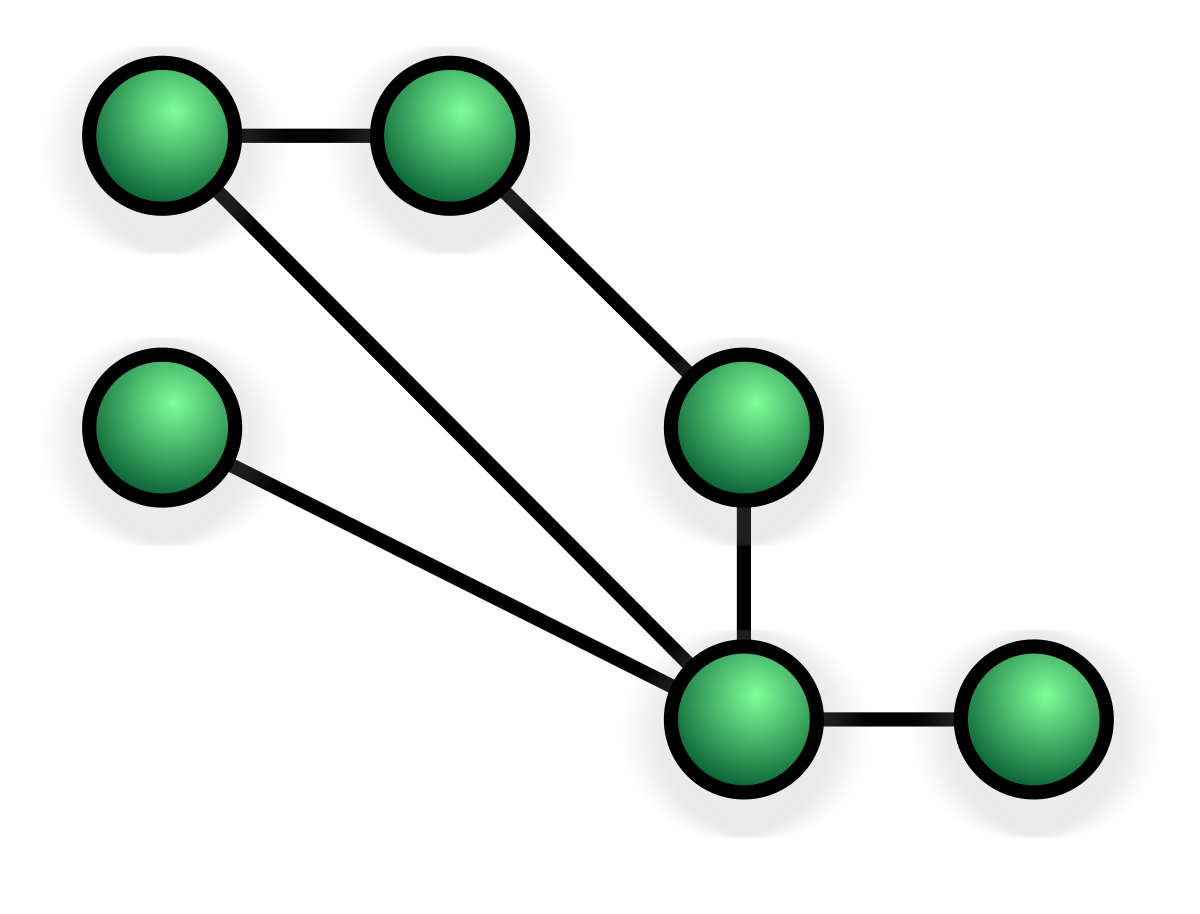
\includegraphics[scale=0.1]{mesh_partial}  
	\caption[Topologi Partially Connected Mesh]{Topologi Partially Connected Mesh} 
	\label{fig:mesh_partial} 
\end{figure} 
\begin{figure} [H]
	\centering  
	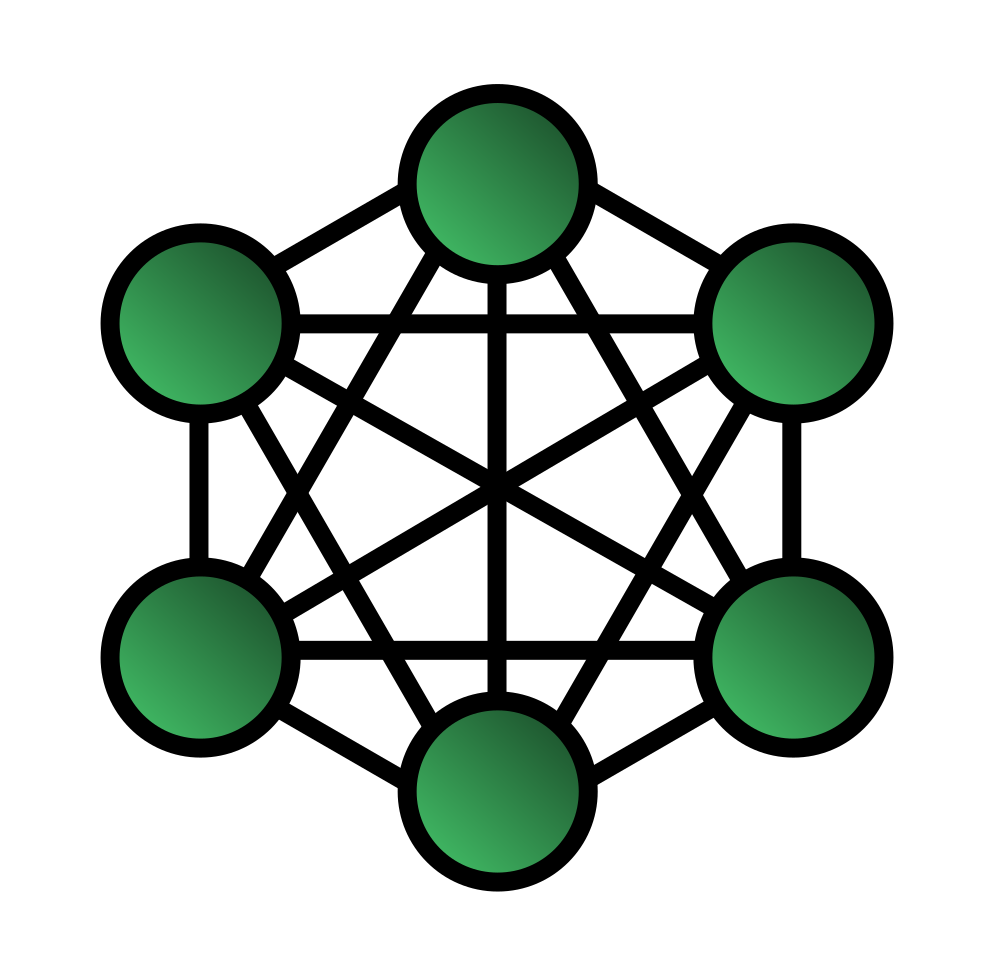
\includegraphics[scale=0.1]{mesh_fully}  
	\caption[Topologi Fully Connected Mesh]{Topologi Fully Connected Mesh} 
	\label{fig:mesh_fully} 
\end{figure} 

Arsitektur yang biasanya dipakai pada WSN adalah \textbf{arsitektur flat / peer-to-peer} dan \textbf{arsitektur hirarkikal}. Selain itu dalam membangun WSN perlu juga diperhatikan jalur komunikasi yang digunakan untuk menghubungkan antar node sensor saat transfer data. Untuk area \textit{sensing} yang tidak terlalu luas dan hanya menggunakan sedikit node sensor dapat menggunakan cara komunikasi \textbf{\textit{single hop}}. Sedangkan untuk daerah yang luas dan memerlukan banyak node sensor dapat menggunakan cara komunikasi \textbf{\textit{multi hop}}. 

\begin{figure} [H]
	\centering  
	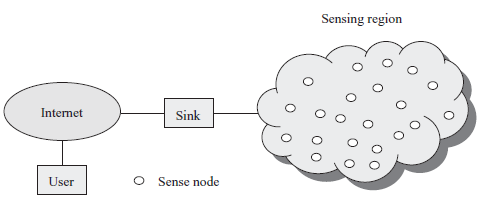
\includegraphics[scale=1]{arsitektur}  
	\caption[Arsitektur Wireless Sensor Network]{Arsitektur Wireless Sensor Network} 
	\label{fig:arsitektur} 
\end{figure} 

\subsubsection{Single-Hop dan Multi-Hop}
Untuk mengirim data ke \textit{sink node} setiap node sensor dapat menggunakan \textit{single-hop long-distance transmission}. \textit{Single-hop long-distance} ini berarti setiap node sensor akan mengirimkan data ke sink node hanya satu kali lompatan walaupun jarak antara sink node dengan node sensor itu sangat jauh. Dalam jaringan sensor, penggunaan energi paling besar adalah saat melakukan komunikasi dibandingan saat sensing. Penggunaan energi akan semakin bertambah jika jarak sink dan node sensor semakin jauh. Untuk menangani masalah tersebut muncul protokol \textit{multi-hop}.

Pada protokol \textit{multi-hop}, node sensor akan disusun saling berdekatan dan terhubung dengan yang lain. Jadi saat akan berkomunikasi dengan \textit{sink node}, node sensor harus mengirimkan data tersebut ke node sensor tetangganya dan diteruskan hingga sampai ke \textit{sink node}. Karena jarak yang saling berdekatan maka penggunaan energi dapat efektif. \textit{Single-hop} dan \textit{multi-hop} ini dapat digunakan pada topologi flat maupun hirarkikal sesuai dengan kebutuhan sistem.

\subsubsection{Arsitektur Flat / Peer-to-Peer}
Pada arsitektur flat, setiap node sensor memiliki peran atau \textit{role} yang sama dalam melakukan \textit{sensing}. Secara fungsional hanya terdapat dua macam node sensor pada arsitektur flat, yaitu \textit{source node} dan \textit{sink node}. Untuk mendapatkan data dilakukan dengan cara \textit{sink node} melakukan pengiriman data ke semua node sensor pada area \textit{sensing} dengan cara \textit{flooding} dan hanya node sensor yang sesuai yang akan merespon \textit{sink node}. Setiap node sensor mengirimkan data ke \textit{sink node} dengan \textit{multi hop} dan melalui node tetangganya yang terhubung dengannya untuk meneruskan data (Gambar~\ref{fig:flat}).
% gambar flat
\begin{figure} [H]
	\centering  
	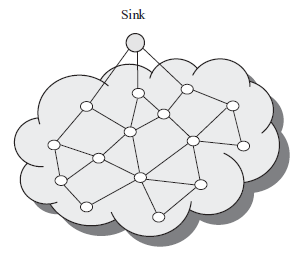
\includegraphics[scale=0.7]{flat}  
	\caption[Arsitektur flat pada \textit{Wireless Sensor Network}]{Arsitektur flat pada \textit{Wireless Sensor Network}} 
	\label{fig:flat} 
\end{figure} 

\subsubsection{Arsitektur Hirarkikal}
Pada arsitektur hirarkikal, semua node sensor dikelompokan ke dalam cluster-cluster. Terdapat \textit{cluster head} pada setiap cluster. \textit{Cluster head} ini yang mengumpulkan data dari setiap node sensor di bawahnya dan meneruskan data yang telah diterima ke \textit{base station} atau \textit{sink node}. Hal yang perlu diperhatikan pada arsitektur hirarkikal adalah pemilihan node sensor sebagai \textit{cluster head} dan node sensor yang melakukan sensing. Penggunaan energi yang paling besar dalam WSN ini adalah saat melakukan komunikasi yaitu saat mengirimkan data ke node sensor lain. Maka untuk node sensor yang memiliki energi kecil dapat digunakan untuk \textit{sensing}, karena node sensor ini hanya melakukan komunikasi ke \textit{cluster head}. \textit{Cluster head} harus memiliki energi atau daya yang lebih banyak, karena \textit{cluster head} akan bertugas menerima hasil sensing node sensor di bawahnya dan meneruskan data ke \textit{sink node}. 

Masalah yang utama pada clustering ini adalah pemilihan \textit{cluster head} dan bagaimana cara mengatur setiap cluster. Terdapat beberapa cara untuk membuat clustering ini. Bedasarkan jarak antara \textit{cluster head} dengan cluster member, dapat dibuat clustering dengan \textit{single-hop} atau \textit{multi-hop} seperti pada Gambar~\ref{fig:cluster_single} dan Gambar~\ref{fig:cluster_multi}. Sedangkan jika berdasarkan jumlah \textit{tier} atau tingkat dapat dibangun \textit{clustering single tier} atau \textit{multi tier} (Gambar~\ref{fig:cluster_multitier}).
\begin{figure} [H]
	\centering  
	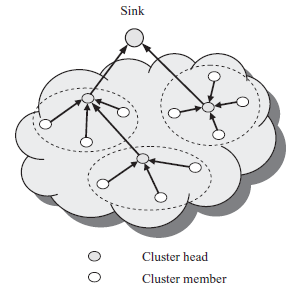
\includegraphics[scale=0.8]{cluster_single}  
	\caption[Arsitektur hierarki pada \textit{Wireless Sensor Network} dengan \textit{single hop} terhadap \textit{Cluster Head}]{Arsitektur hierarki pada \textit{Wireless Sensor Network} dengan \textit{single hop} terhadap \textit{Cluster Head}} 
	\label{fig:cluster_single} 
\end{figure} 
\begin{figure} [H]
	\centering  
	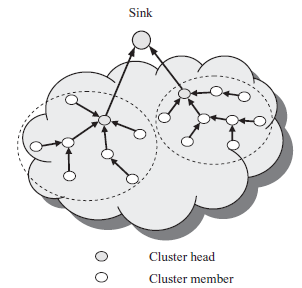
\includegraphics[scale=0.8]{cluster_multi}  
	\caption[Arsitektur hierarki pada \textit{Wireless Sensor Network} dengan \textit{multi hop}]{Arsitektur hierarki pada \textit{Wireless Sensor Network} dengan \textit{multi hop}} 
	\label{fig:cluster_multi} 
\end{figure} 
\begin{figure} [H]
	\centering  
	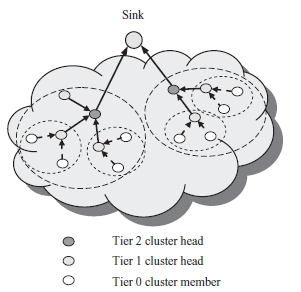
\includegraphics[scale=0.8]{cluster_multitier}  
	\caption[Clsutering dengan multi tier]{Clsutering dengan multi tier} 
	\label{fig:cluster_multitier} 
\end{figure}

%00 wireless sensor network hal 293
\subsection{Sistem Operasi}
Setiap node sensor memerlukan sistem operasi (OS) untuk mengontrol perangkat keras dan perangkat lunak. Sistem operasi tradisional tidak dapat digunakan pada WSN. Pada sistem operasi tradisional digunakan untuk mengatur proses, memori, CPU, dan sistem berkas. Terdapat beberapa hal yang harus ditangani oleh sistem operasi dalam WSN yaitu:
\begin{enumerate}
	\item WSN memerlukan \textit{real-time scheduler}. Data yang didapat harus segera dikirim atau diproses.
	\item Pengaturan memori karena memori pada WSN sangat kecil.
	\item Pengaturan data yang efisien terkait dengan \textit{microprocessor} dan memori yang terbatas
	\item Mendukung kode pemrograman yang efisien dan \textit{reliable} karena dapat terjadi perubahan kode saat implementasi.
	\item Mendukung pengaturan sumber daya untuk menambah waktu hidup dari node sensor dan meningkatkan performa dengan \textit{sleep time} saat tidak ada kegiatan atau \textit{wake up time} saat terdapat interupsi dari lingkungan.
	\item Mendukung antarmuka untuk pemrograman dan antarmuka perangkat lunak. 
\end{enumerate}

Beberapa sistem operasi yang umum digunakan pada WSN antara lain :
\begin{enumerate}
	\item TinyOS
	\item Contiki
	\item LiteOS
	\item PreonVM
\end{enumerate}

%Operating SYstem for WSN a survey - hal 7
\subsubsection{TinyOS}
TinyOS adalah sistem operasi \textit{open-source} yang digunakan pada WSN. TinyOS dapat menjalankan program dengan memori yang sangat kecil. Ukurannya hanya 400 Byte. Komponen \textit{library} TinyOS terdiri dari protokol jaringan, layanan distribusi sensor, \textit{driver sensor}, dan perangkat lunak pengamatan data sensor yang dapat digunakan untuk melakukan monitoring jaringan sensor. Gambar~\ref{fig:tinyOS} adalah arsitektur pada TinyOS. 
\begin{figure} [H]
	\centering  
	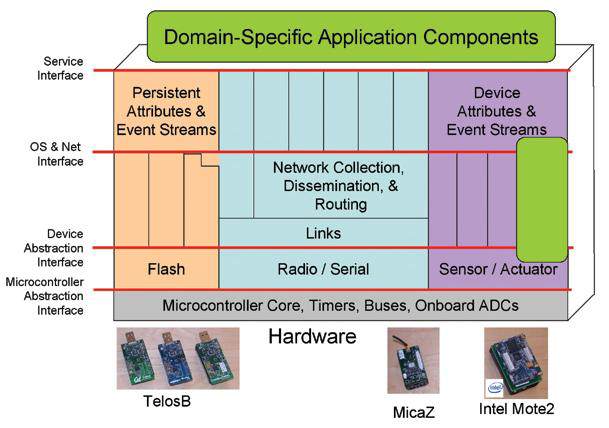
\includegraphics[scale=0.5]{tinyOS}  
	\caption[Arsitektur TinyOS]{Arsitektur TinyOS} 
	\label{fig:tinyOS} 
\end{figure}

%Operating SYstem for WSN a survey - hal 11
\subsubsection{Contiki}
Contiki adalah sistem operasi \textit{open-source} dengan Bahasa Pemrograman C yang digunakan pada WSN. Pengaturan Contiki hanya memerlukan 2KB dari RAM dan 40KB dari ROM. Fitur yang dimiliki oleh Contiki antara lain: \textit{multitasking}, \textit{multithreading}, jaringan TCP/IP, IPv6, GUI, \textit{Web Browser}, \textit{Web Server}, telnet, dan komputasi jaringan virtual. Gambar~\ref{fig:contiki} adalah arsitektur pada Contiki
\begin{figure} [H]
	\centering  
	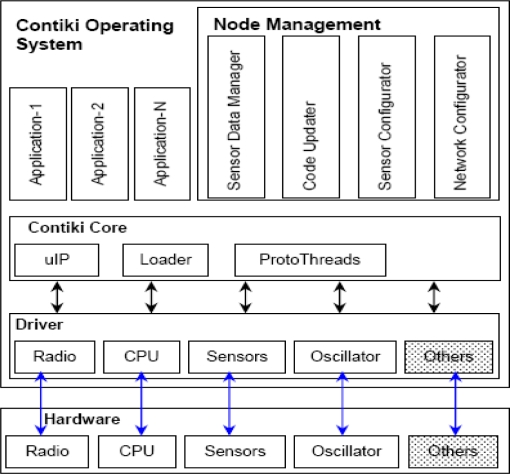
\includegraphics[scale=3]{contiki}  
	\caption[Arsitektur Contiki]{Arsitektur Contiki} 
	\label{fig:contiki} 
\end{figure}

%Operating SYstem for WSN a survey - hal 23
\subsubsection{LiteOS}
LiteOS adalah sistem operasi mirip UNIX yang didisain untuk WSN. Tujuan dibuat LiteOS adalah membuat sistem operasi yang mirip dengan UNIX agar lebih lebih familiar dengan paradigma pemrograman UNIX. Pada LiteOS terdapat sistem berkas yang hiearki, dan mendukung Bahasa Pemrograman LiteC++ dan UNIX Shell. LiteOS dapat digunakan untuk MicaZ yang memiliki 8 Mhz CPU, 128 byte flash, dan 4KB RAM. LiteOS memiliki tiga komponen utama yaitu: LiteShell, LiteFS, dan Kernel. Gambar~\ref{fig:contiki} adalah arsitektur pada LiteOS
\begin{figure} [H]
	\centering  
	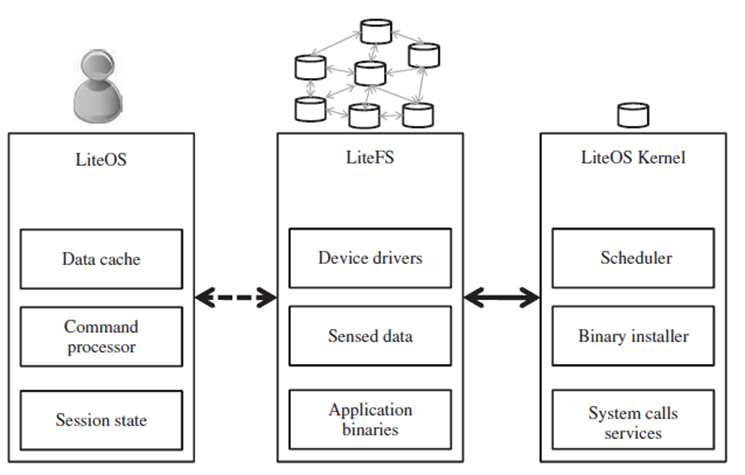
\includegraphics[scale=0.4]{liteOS}  
	\caption[Arsitektur LiteOS]{Arsitektur LiteOS} 
	\label{fig:liteOS} 
\end{figure}

Perbandingan dari TinyOS, Contiki, dan LiteOS dapat dilihat pada Tabel~\ref{tab:perbandinganOS} berikut ini:
\begin{table}[H] %atau h saja untuk "kira kira di sini"
	\centering 
	\caption{Tabel Perbandingan Sistem Operasi}
	\label{tab:perbandinganOS}
	\begin{tabular}{| p{1.6cm} | p{3.8cm} | p{2.5cm} | p{3cm} | p{4cm} |}
		\toprule
		OS & Programming Paradigm & Scheduling & Memory Allocation & System Call\\ 
		
		\midrule
		TinyOS & Event-based & FIFO & Static & Not Available\\
		Contiki & Predominant event-based & FIFO & Dynamic & Runtime libraries\\ 
		LiteOS & Thread-based & Priority-based scheduling with optional round-robin support & Dynamic & A host of system calls available to the user (file, process, environment, debugging, and device command) 	\\ 

		\bottomrule
		
	\end{tabular} 
\end{table}

%data transfer 
\subsection{Protokol Stack pada Wireless Sensor Network}
WSN memiliki lima layer protokol: physical layer, data link layer, network layer, transport layer, dan application layer, seperti pada Gambar~\ref{fig:layer}. 

\begin{figure} [H]
	\centering  
	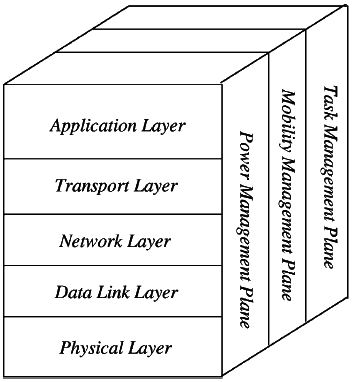
\includegraphics[scale=0.5]{layer}  
	\caption[Layer pada \textit{Wireless Sensor Network}]{Layer pada \textit{Wireless Sensor Network}} 
	\label{fig:layer} 
\end{figure} 

Selain itu protokol stack pada WSN dibagi kedalam 3 grup manajemen yaitu \textit{power management plane}, \textit{connection management plane}, dan \textit{task management plane}. \textbf{\textit{Power Management Plane}} bertanggung jawab untuk melakukan manajemen sumber daya atau energi pada setiap node sensor saat melakukan sensing, processing, transfer data dan menerima data. Contohnya pada layer MAC node sensor dapat mematikan transceiver saat tidak ada data untuk dikirim dan diterima. Pada \textit{network layer}, node sensor dapat memilih node sensor tetangga saat akan melakukan transfer data agar penggunaan energi yang minimal. \textbf{\textit{Connection Management Plane}} bertanggung jawab untuk melakukan pengaturan terhadap node sensor terkait dengan koneksi antar node sensor. \textbf{\textit{Task Management Plane}} bertanggung jawab untuk mengatur distribusi tugas atau \textit{task} pada node sensor dalam melakukan \textit{sensing} agar tercapai penggunaan energi yang efisien.

\subsubsection{Physical Layer}
\textit{Physical layer} bertanggung jawab untuk mengubah bit stream dari data link layer menjadi sinyal agar bisa dilakukan transmisi melalui media komunikasi yang terdapat (transceiver). Pemilihan media dan frekuensi adalah hal yang penting dalam komunikasi antar node sensor. Salah satu cara yang bisa digunakan adalah dengan menggunakan \textit{Radio frequency} (RF). Jaringan sensor memerlukan biaya yang kecil, ukuran yang kecil, dan penggunaan daya yang kecil untuk tranceivernya. Karena itu banyak yang menggunakan Radio Frequency (RF) untuk desain perangkat keras node sensornya.

%pengertian multiplexing
\subsubsection{Data Link Layer}
\textit{Data link layer} bertanggung jawab untuk melakukan \textit{multiplexing} pada aliran data, membentuk data frame, mendeteksi data frame, \textit{medium access}, dan mengatur kesalahan saat transmisi data. Fungsi paling penting data link layer adalah \textit{Medium Access Control} (MAC). Protokol MAC menentukan kapan node sensor mengakses media untuk mengirim data, melakukan kontrol dan mengatur paket ke node sensor lain. Hal itu dilakukan agar tidak terjadi paket yang bertabrakan. 

\subsubsection{Network Layer}
\textit{Network layer} bertanggung jawab untuk \textit{routing} dari node sensor ke \textit{sink node}. Pada WSN node sensor tersebar pada suatu tempat untuk melakukan \textit{sensing}. Data hasil \textit{sensing} tersebut harus dikirimkan ke \textit{sink node} untuk diolah. Dalam mengirimkan data tersebut dapat menggunakan \textit{single-hop} atau \textit{multi hop}. Dalam mengirim data diperlukan protokol routing yang tepat agar hemat energi.

\subsubsection{Transport Layer}
Secara umum \textit{transport layer} bertanggung jawab untuk pengiriman data yang \textit{reliable} antara node sensor dan \textit{sink node}. Protokol transpor yang biasa pada jaringan komputer tidak bisa diterapkan pada WSN tanpa modifikasi. Setiap jaringan sensor memiliki fungsi khusus. Untuk aplikasi yang berbeda memerlukan kebutuhkan reliabilitas yang berbeda. Pengiriman data pada WSN dibagi menjadi dua yaitu: \textbf{\textit{downstream}} dan \textbf{\textit{upstream}}. \textbf{\textit{Upstream}} berarti node sensor mengirimkan hasil sensing ke sink node. \textbf{\textit{Downstream}} berarti data berasal dari sink node contohnya, kueri, dan perintah-perintah yang dikirimkan ke setiap node sensor. Aliran data yang \textit{reliable} untuk kedua jenis pengiriman ini berbeda. Pada \textit{upstream}, \textit{reliable} data dapat ditoleransi karena sensor akan melakukan sensing terus menerus dan dapat terjadi pengulangan data sehingga data yang hilang tadi dapat dikoreksi. Sedangkan pada \textit{downstream} memerlukan 100\% pengiriman data yang \textit{reliable} karena aplikasi tidak dapat berjalan jika kode program tidak lengkap. 

%query dissemination GAK TAU APAAN
\subsubsection{Application Layer}
\textit{Application layer} meliputi berbagai macam protokol yang ada pada layer ini untuk menjalankan berbagai macam aplikasi seperti \textit{query dissemination}, \textit{node localization}, \textit{time synchronization}, dan \textit{network security}. Protokol yang ada pada layer ini antara lain:
\begin{enumerate}
	\item Sensor management protocol (SMP) adalah protokol untuk melakukan pertukaran lokasi data, sinkornisasi node sensor, mengatur ulang node sensor, dan menyimpan status dari node sensor.
	\item Sensor query and data dissemination protocol (SQDDP) adalah protokol yang mendukung antarmuka aplikasi untuk memasukan query, merespon query, dan mengumpulkan respon.
	\item Sensor query and tasking language (SQTL) adalah protokol untuk mendukung bahasa pemrograman pada WSN.
\end{enumerate}


% http://profsite.um.ac.ir/~hyaghmae/WSN/transport.pdf
\section{Reliable Data Transfer di WSN}
WSN terdiri dari \textit{sink node} dan banyak node sensor. Saat melakukan sensing dan mengirim data ke \textit{sink node}, semua node sensor akan mengirimkan data melalui media yang sama. Hal ini dapat membanjiri jaringan dengan data tersebut dan menyebabkan \textit{congestion} atau kemacetan pada jaringan yang berakibat \textit{data loss} atau hilang. Untuk menangani \textit{data loss}, maka dalam membangun WSN adalah salah satu yang diperlukan adalah protokol yang menangani \textit{Reliability}. \textit{Reliability} berarti memastikan data yang dikirim dari setiap node sensor diterima oleh \textit{base station} secara lengkap dan sesuai dengan urutan pengiriman.

\subsection{Jenis Reliability}
Berdasarkan tingkat, reliability ada dua macam yaitu:
\begin{enumerate}
	\item Packet Reliability
	\item Event Reliability
\end{enumerate}  
\subparagraph{Packet Reliability} berarti paket yang dikirim harus sampai kepada tujuan (\textit{base station}) secara utuh. \textit{Packet reliability} ini membutuhkan \textit{acknowledge} dari node sensor. Tantangan yang harus dihadapi dari \textit{packet reliability} adalah dalam mengirim ulang paket yang hilang akan menghabiskan energi atau daya.
\subparagraph{Event Reliability} berarti hanya data hasil \textit{sensing} yang akan dikirim ke \textit{base station}. Pada \textit{Event reliability} tidak membutuhkan \textit{acknowledge}. Karena data yang hilang itu tidak banyak berpengaruh sehingga tidak dibutuhkan pengiriman ulang (\textit{retransmission}) data.

Berdasarkan arah, \textit{reliability} ada dua macam yaitu:
\begin{itemize}
	\item Upstream Reliability
	\item Downstream Reliability
\end{itemize}
\subparagraph{Upstream Reliability} adalah komunikasi dari node sensor ke \textit{sink node}. Banyak protokol yang mendukung \textit{upstream reliability}. Pengiriman data yang dilakukan adalah \textit{unicast} yang berarti hanya dari satu titik ke titik lain.
\subparagraph{Downstream Reliability} adalah adalah komunikasi dari \textit{sink node} ke node sensor. Pengiriman data biasanya dilakukan dengan cara \textit{broadcast} ke semua node sensor. Data yang dikirim ini biasanya adalah kode program untuk melakukan \textit{sensing}. 

Pada protokol transport tradisional dikenal istilah TCP dan UDP, namun keduanya tidak bisa diimplementasikan pada WSN. Namun, protokol transport tersebut bisa dibuat dengan beberapa pertimbangan seperti:
\begin{itemize}
	\item WSN membutuhkan mekanisme untuk mengembalikan paket yang hilang seperti \textit{acknowledge}.
	\item Proses awal dalam membangun koneksi seperti \textit{handshake} harus disederhanakan karena akan membuang banyak daya atau energi.
	\item Protokol harus dapat menangani \textit{congestion}.
	\item Protokol harus dapat adil terhadap setiap node sensor seperti pembagian penggunaan jaringan. (\textit{bandwidth})
\end{itemize} 

\textit{Retransmission} dapat dilakukan dengan \textit{End-to-End Retransmission} dan \textit{Hop-by-Hop Retransmission (Link Level Retransmission)}. Pada \textbf{\textit{End-to-End transmission}} dan terjadi \textit{data loss}, maka pengirim harus mengirim ulang semua paket dan akan menghabiskan lebih banyak daya. \textit{End-to-End Retransmission} adalah salah satu metode yang digunakan di Internet. Cara ini dapat memastikan \textit{reliable} data tanpa harus mengetahui apa yang terjadi di tengah jaringan. Pada \textit{End-to-End Retransmission} diperlukan \textit{handshake} seperti pada komunikasi jaringan komputer. Pada awalnya data dikirim sebagai permintaan transfer. Jika penerima (\textit{receiver}) memiliki cukup RAM, dan layer aplikasi dapat menerima data tersebut, maka \textit{receiver} mengirimkan \textit{acknowledge} untuk permintaan data tersebut. Saat koneksi sudah terbentuk, data yang sebenarnya dapat dikirim. Data tersusun dari beberapa \textit{round}. Setiap \textit{round}, pengirim (\textit{sender}) mengirim paket yang hilang pada round sebelumnya. Diakhir setiap  round, \textit{receiver} mengirimkan \textit{acknowledge} kepada \textit{sender} yang berisi informasi paket yang hilang. \textit{Sender} menerima \textit{acknowledge} tersebut dan mengirim paket yang hilang tersebut. Untuk round pertama terdapat pengecualian karena semua pake pada round sebelumnya tidak ada (belum dikirim). 

Sedangkan pada \textbf{\textit{hop-by-hop transmission}} dilakukan antara node sensor dengan node sensor tetangganya. Jadi saat terjadi \textit{data loss} maka pengiriman ulang lebih sedikit dalam menghabiskan daya. \textit{Hop-by-hop} ini membutuhkan \textit{buffer} atau penyimpanan sementara pada setiap node sensor dan lebih efektif dilakukan pada topologi WSN \textit{multi-hop}. Buffer ini digunakan untuk menyimpan data sementara hingga mendapatkan \textit{acknowledge} dari hop berikutnya.

\subsection{Jenis - jenis Acknowledge}
Dalam mencapai reliability dapat digunakan acknowledge saat melakukan pengiriman data. Terdapat empat jenis acknowledge yang dapat digunakan, yaitu:
\begin{enumerate}
	\item Explicit Acknowledge (eACK) : Penerima memberitahu pengirim bahwa paket telah diterima dengan tepat sekaligus memberitahu pengirim paket mana yang belum diterima untuk dilakukan \textit{retransmission}.
	\item Negative Acknowledge (nACK) : Penerima memberitahu pengirim bahwa paket yang diterima tidak benar dan diperlukan \textit{retransmission}.
	\item Implicit Acknowledge (iACK) : Setelah pengirim mengirim pesan, pengirim akan memastikan paket data dikirim ke tetangganya memberikan acknowledge.
	\item Selective Acknowledge (sACK) : Hanya paket yang hilang dari sebuah pesan yang akan dikirim ulang
\end{enumerate}

\subsection{Protokol Transport yang Reliable}
Ada banyak protokol untuk memastikan \textit{reliability} pada WSN. Beberapa protokol mendukung \textit{upstream,} dan beberapa protokol mendukung \textit{downstream}. Hanya ada sedikit protokol yang dapat mendukung keduanya. Selain itu ada protokol yang memiliki fokus utama untuk menangani \textit{reliability} saja dan ada yang menangani \textit{congestion} sekaligus \textit{reliability}. 

Beberapa protokol transport yang sering digunakan antara lain:
\begin{itemize}
	\item GARUDA
	\item Event-to-Sink Reliable Transport (ESRT)
	\item Reliable Multi Segment Transport (RMST)
	\item Pump Slowly Fetch Quickly (PSFQ)
	\item Asymmetric Reliable Transport (ART)
	\item Price Oriented Reliable Transport (PORT)
	\item Delay Sensitive Transport (DST)
\end{itemize}

\subsubsection{GARUDA}
GARUDA adalah salah satu protokol \textit{downstream} yang menggunakan \textit{hop-by-hop retransmission}. GARUDA menggunakan mekanisme NACK untuk mendeteksi paket yang hilang. GARUDA dan tidak menangani \textit{congestion}. GARUDA menggunakan mekanisme WFP (Wait for First Packet) pulse transmission.

\subsubsection{Event-to-Sink Reliable Transport}
Event-to-Sink Reliable Transport (ESRT) adalah protokol \textit{upstream} yang lebih banyak digunakan untuk mengirim event dibandingkan paket data. Pada ESRT tingkat pengiriman pada setiap node sensor bergantung pada tingkat reliabilitas di \textit{sink node} dan dengan status jaringan tersebut (terdapat kemacetan atau tidak). ESRT adalah protokol pertama yang menangani \textit{congestion control} dan \textit{reliability} sekaligus. Pada ESRT setiap node sensor mendeteksi \textit{congestion} berdasarkan peningkatan \textit{buffer} lalu menambahkan N bit pada \textit{header} sebuah paket dan meneruskannya ke sink node. Berdasarkan paket yang diterima oleh \textit{sink node}, dapat diketahui keadaan dari jaringan dan juga \textit{reliability} suatu paket untuk menentukan jumlah paket yang telah berhasil diterima pada periode tertentu. ESRT tidak menggunakan ACK/NACK untuk mendeteksi data yang hilang, karena menyebabkan penggunaan energi yang sangat besar.

\subsubsection{Reliable Multi Segment Transport}
Reliable Multi Segment Transport (RMST) adalah protokol \textit{upstream} yang menggunakan \textit{selective NACK} untuk memastikan paket yang \textit{loss} dan mengirim ulang paket tersebut. RMST ini menggunakan \textit{timer} untuk mendeteksi paket yang \textit{loss}. RMST ini tidak menangani \textit{congestion control} dan masalah terkait penggunaan energi.

\subsubsection{Pump Slowly Fetch Quickly}
Pump Slowly Fetch Quickly (PSFQ) adalah protokol \textit{downstream}. Cara kerja PSFQ adalah dengan memasukan paket kedalam jaringan (\textit{Pump Operation}). Saat terjadi \textit{data loss}, protokol ini akan menjalankan pemulihan \textit{hop-by-hop}. PSFQ menggunakan NACK. Protokol ini tidak mendukung \textit{congestion control} dan \textit{paket loss} secara satuan.

\subsubsection{Asymmetric Reliable Transport}
Asymmetric Reliable Transport (ART) adalah protokol yang berbasis pada \textit{event} dan \textit{query reliability}. ART merupakan protokol \textit{bidirectional} pertama yang sudah mendukung \textit{congestion control}. Terdiri dari kumpulan node yang disebut \textit{essential node} yang tersebar pada suatu area untuk melakukan \textit{sensing} dan beberapa node yang disebut \textit{non-essential node} yang terlibat pada pengiriman data dan \textit{congestion control}.

\subsubsection{Price Oriented Reliable Transport}
Price Oriented Reliable Transport Protocol (PORT) adalah protokol \textit{upstream} yang berbasis pada \textit{event reliability} dengan penggunaan energi seminimal mungkin. PORT mendukung mekanisme dengan energi yang efisien disertai \textit{congestion control}. Selain itu PORT juga adalah protokol yang mendukung komunikasi \textit{End-to-End}. PORT membutuhkan \textit{sink node} untuk mengatur aliran data. Kekurangannya adalah tidak ada pemulihan paket yang hilang.

\subsubsection{Delay Sensitive Transport}
Delay Sensitive Transport (DST) adalah tambahan dari ESRT. Tujuan dari DST adalah dicapai \textit{reliability} pada \textit{sink node}. Pada DST terdapat aturan \textit{Time Critical Event First} (TCEF).TCEF berarti data paket dengan diberikan prioritas untuk melakukan \textit{retransmission}. DST dapat bekerja dengan baik pada satu event, namun pada banyak event akan menjadi lebih kompleks.
\\
\\
Lebih singkat setiap protokol tersebut dapat dilihat pada Tabel~\ref{tab:protokol_reliable}
\begin{table}[H] %atau h saja untuk "kira kira di sini"
	\centering 
	\caption{Tabel Perbandingan Protokol}
	\label{tab:protokol_reliable}
	\begin{tabular}{|c|c|c|c|c|c|c|}
		\toprule
		Protokol & Arah & Tingkat & Mekanisme & Tipe ACK & Menangani Congestion & Energi Efisien \\

		\midrule
		GARUDA & Downstream & Packet & Hop-By-Hop & NACK & Tidak & Tidak\\
		ESRT & Upstream & Event & End-to-End & - & Ya & Ya\\
		RMST & Upstream & Packet & Hop-By-Hop & NACK & Tidak & Ya\\
		PSFQ & Downstream & Packet & Hop-By-Hop & NACK & Tidak & Tidak\\
		ART & Both & Event & End-to-End	 & - & Ya & Ya\\
		PORT & Upstream & Event & Hop-By-Hop & - & Ya & Ya\\
		DST & Upstream & Event & End-to-End & - & Tidak & Ya\\

		\bottomrule
		
	\end{tabular} 
\end{table}

\section{PreonVM}
\label{sec:PreonVM}
PreonVM adalah virtual machine (VM) yang dibuat oleh VIRTENIO untuk sistem komputer yang dirancang khusus (\textit{embedded system}) dengan sumber daya yang terbatas. PreonVM dapat digunakan pada node sensor jenis Preon32. PreonVM dibuat sangat optimal dengan tidak dibutuhkannya sistem operasi tambahan dan berjalan langsung pada \textit{microprocessor}. Dengan PreonVM ini \textit{developer} dapat membuat aplikasi dengan mudah pada Bahasa Java yang mengumpulkan data dari sensor dan mengontrol aktuator. API pada PreonVM mendukung antarmuka radio sesuai dengan IEEE 802.15.4 dan AES encryption pada perangkat kerasnya. 

PreonVM memiliki fitur sebagai berikut:
\begin{itemize}
	\item Aplikasi dibangun dengan Bahasa Pemrograman Java
	\item Mendukung semua tipe data pada Java seperti char, byte, int, long, float atau double
	%Garbage collection adalah program yang berjalan pada java virtual machine untuk menyingkirkan object yang tidak dibutuhkan pada aplikasi.
	\item \textit{Garbage collection} dengan \textit{memory defragmentation}
	\item Mendukung \textit{exception handling}, stack dan array multidimensi
	\item Terdapat \textit{system properties} untuk mengatur aplikasi
	\item Tidak membutuhkan sistem operasi tambahan
	\item Mendukung threads termasuk synchronized, Object.wait, Object.notify, Object.notifyAll, Thread.sleep, Thread.interrupt
\end{itemize}

Kelebihan yang dimiliki oleh VIRTENIO ini adalah \textit{object-oriented programming} dengan Bahasa Pemrograman Java. VIRTENIO menyediakan virtual machine sebagai sistem operasi yang inovatif untuk modul Preon32. Dengan menggunakan virtual machine, aplikasi dapat berdiri sendiri pada arsitektur yang dibuat. Dengan demikian aplikasi Java yang dibuat dapat dijalankan pada aristektur yang berbeda tanpa harus modifikasi. Gambar~\ref{fig:PreonVM} menunjukan ilustrasi penggunaan virtual machine pada berbagai perangkat. 

\begin{figure} [H]
	\centering  
	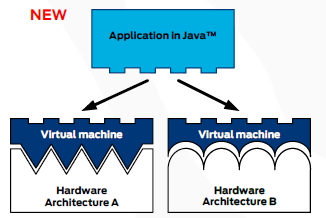
\includegraphics[scale=0.7]{PreonVM}  
	\caption[Penggunaan virtual machine pada perangkat yang berbeda]{Penggunaan virtual machine pada perangkat yang berbeda} 
	\label{fig:PreonVM} 
\end{figure} 

Virtual machine juga membatu memisahkan proses pengembangan perangkat keras dengan aplikasi perangkat lunak. Program aplikasi dikembangan dengan antarmuka yang abstrak dan tidak berubah. Sebagai tambahan, virtual mesin berjalan optimal untuk aplikasi kecil pada 8-bit sampai 32-bit microprocessor dengan 8 Kbyte RAM dan 128 Kbyte Flash.  

\subsection{Preon32}
Preon32 adalah salah satu jenis node sensor. Preon32 menggunakan PreonVM sebagai sistem operasi. Preon32 versi umum memiliki 5 jenis sensor pada sebuah board. Sensor yang ada pada Preon32 ini antara lain sensor suhu (temperature), sensor cahaya, sensor kelembapan udara (humidity), sensor untuk mengukur tekanan udara (barometer), dan sensor getaran. Pada versi tambahan Preon32 dapat dilengkapi dengan sensor untuk mendeteksi medan magnet (magnetometer), dan gyroscope. Semua jenis sensor tersebut dapat diatur melalui PreonVM dan pemrograman dapat dilakukan dengan Bahasa Pemrograman Java. Gambar~\ref{fig:Preon32board} adalah board dan sensor-sensor pada Preon32.
\begin{figure} [H]
	\centering  
	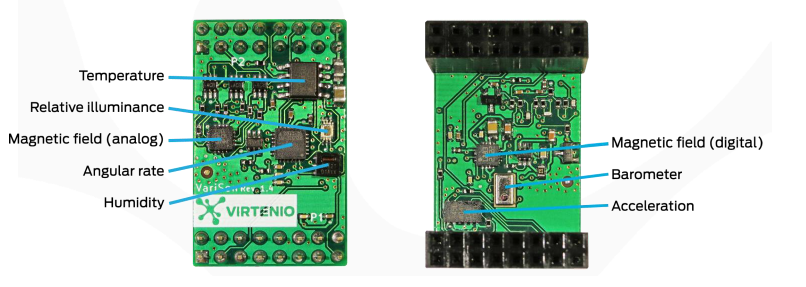
\includegraphics[scale=0.7]{Preon32board}  
	\caption[Preon32 Board]{Preon32 Board} 
	\label{fig:Preon32board} 
\end{figure} 

Preon32 ini dapat diaplikasikan pada berbagai hal seperti:
\begin{enumerate}
	\item Home Automation yang digunakan untuk mengintegrasikan berbagai sistem pada rumah, monitoring area, dan navigasi.  
	\item Platform untuk membantu penelitian
	\item Implementasi aplikais baru pada jaringan nirkabel
	\item Algoritma untuk sensor data fusion
\end{enumerate}


%\subsection{Kutipan}
%\label{subs:kutipan} 
%Berikut contoh kutipan dari berbagai sumber, untuk keterangan lebih lengkap, silahkan membaca file referensi.bib yang disediakan juga di template ini.
%Contoh kutipan:
%\begin{itemize}
%	\item Buku:~\cite{berg:08:compgeom} 
%	\item Bab dalam buku:~\cite{kreveld:04:GIS}
%	\item Artikel dari Jurnal:~\cite{buchin:13:median}
%	\item Artikel dari prosiding seminar/konferensi:~\cite{kreveld:11:median}
%	\item Skripsi/Thesis/Disertasi:~\cite{lionov:02:animasi}~\cite{wiratma:10:following}~\cite{wiratma:22:later}
%	\item Technical/Scientific Report:~\cite{kreveld:07:watertight}
%	\item RFC (Request For Comments):~\cite{RFC1654}
%	\item Technical Documentation/Technical Manual:~\cite{Z.500}~\cite{unicode:16:stdv9}~\cite{google:16:and7}
%	\item Paten:~\cite{webb:12:comm}
%	\item Tidak dipublikasikan:~\cite{wiratma:09:median}~\cite{lionov:11:cpoly}
%	\item Laman web:~\cite{erickson:03:cgmodel}  
%	\item Lain-lain:~\cite{agung:12:tango}
%\end{itemize}    
